\chapter{General Kernel Spectral Method}
\label{chap:general-kernel-spectral-method}

\input{chapters/out/General Kernel Spectral Method.md.tex}

\begin{figure}[H]
  \centering
  \label{fig:morse-operator}
  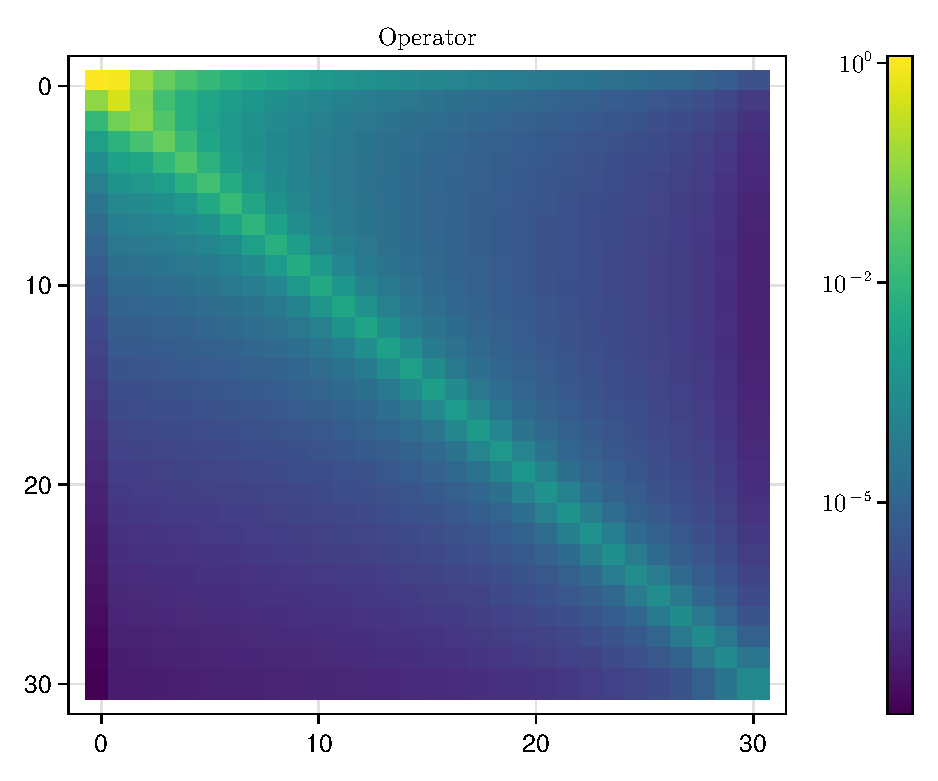
\includegraphics[width=0.5\linewidth]{results/morse-poti/full-operator.pdf}
  \caption{Operator}
\end{figure}

\begin{figure}[H]
  \centering
  \label{fig:morse-solution-increasing-order}
  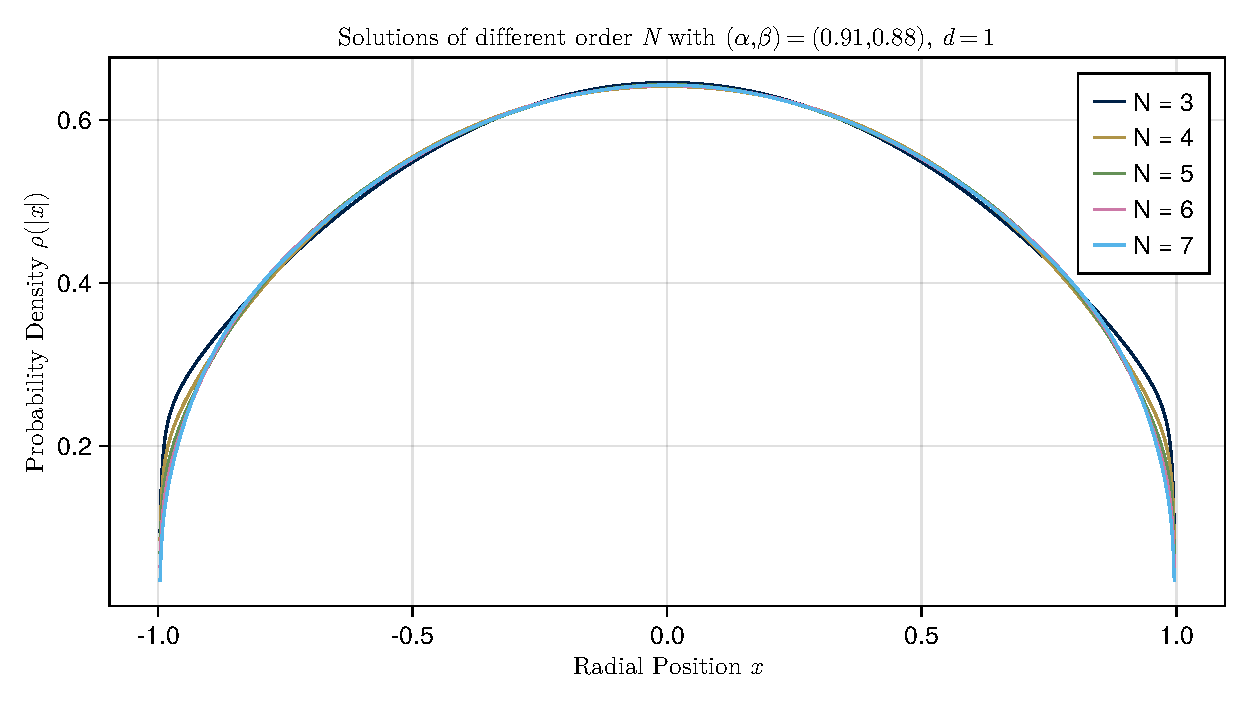
\includegraphics[width=0.8\linewidth]{results/morse-poti/solution-increasing-order.pdf}
  \caption{Solutions of increasing orders}
\end{figure}

\begin{figure}[H]
  \centering
  \label{fig:monomial-basis-convergence}
  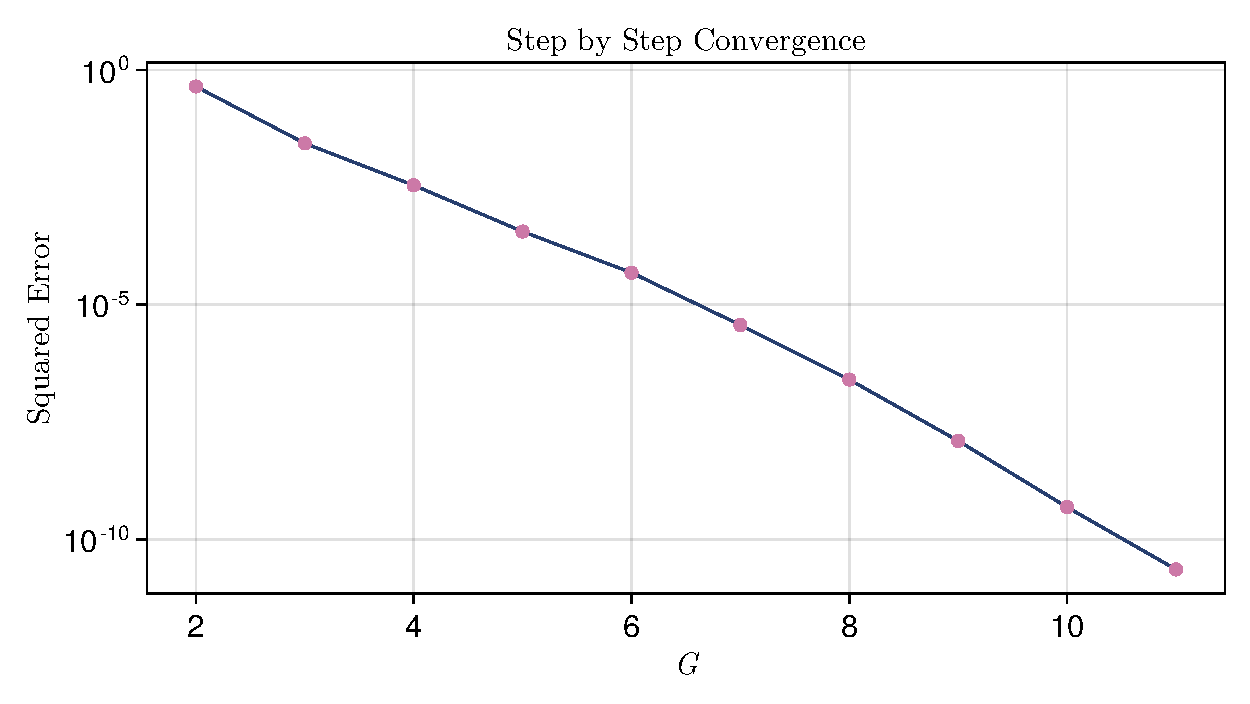
\includegraphics[width=0.7\linewidth]{results/monomial-basis-convergence.pdf}
  \caption{Convergence}
\end{figure}
